\section{实验过程记录}

\subsection{PC设计}
\begin{enumerate}
    \item PC的内核为一个D寄存器,输出为当前指令的地址,输入为下一次指令的地址,可能是PC+4或跳转地址,本实验中默认为PC+4
    \item PC加法器的输入为当前指令的地址和4,输出为PC+4
    \item PC与加法器结合,完成自增操作,能够循环读取下一条指令的地址
\end{enumerate}

\subsection{Controller设计}
\begin{enumerate}
    \item Controller由maindec和aludec组成
    \item 其中maindec负责判断指令类型,并生成相应的控制信号。需实现1个输入,为指令inst的高6位op,输出分为2部分,多个控制信号有作为一个多
    位输出,以及aluop,传输至aludec,使aludec配合inst低6位funct,进行ALU模块控制信号的译码
    \item aludec,负责ALU模块控制信号的译码。输入分别为funct, aluop;输出为alucontrol信号
\end{enumerate}

\subsection{指令存储器调用}
\begin{enumerate}
    \item 根据实验指导书,调用Block Memory,并导入coe文件
\end{enumerate}

\subsection{顶层文件设计}
\begin{enumerate}
    \item 根据单周期CPU数据通路连线情况,将时钟信号模块、程序计数器模块、存储器模块,控制器模块、显示模块连线
    \item 完成对top文件进行仿真,验证单周期CPU取指,译码操作的正确性
    \item 上板验证七段数码管指令循环显示和控制信号在LED上显示是否正常
\end{enumerate}

\subsection{问题及解决方案}

\subsubsection{问题1}
\textbf{问题描述:}在完成所有器件设计后,进行仿真发现控制信号出错

\textbf{解决方案:}从头开始,对PC进行仿真,发现PC无法自增,
原因是将在pc内部调用了加法器,导致加法器连线问题,无法正确仿真,将其放在外面与pc连线后仿真成功(养成好边写边仿真的习惯很重要)

\begin{figure}[htbp]
    \centering
    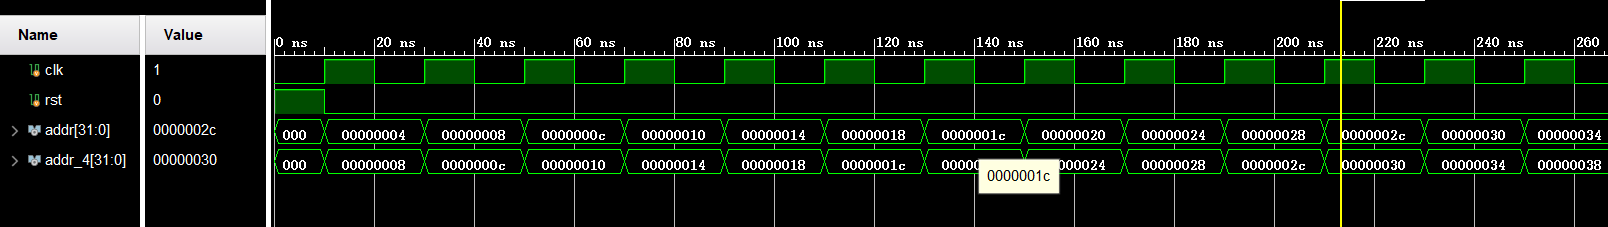
\includegraphics[width=0.8\textwidth]{pc.png}
    \caption{PC}
\end{figure}

\subsubsection{问题2}
\textbf{问题描述:}在解决问题1的基础上,加入存储器进行仿真,发现并没有连续取出指令

\begin{figure}[htbp]
    \centering
    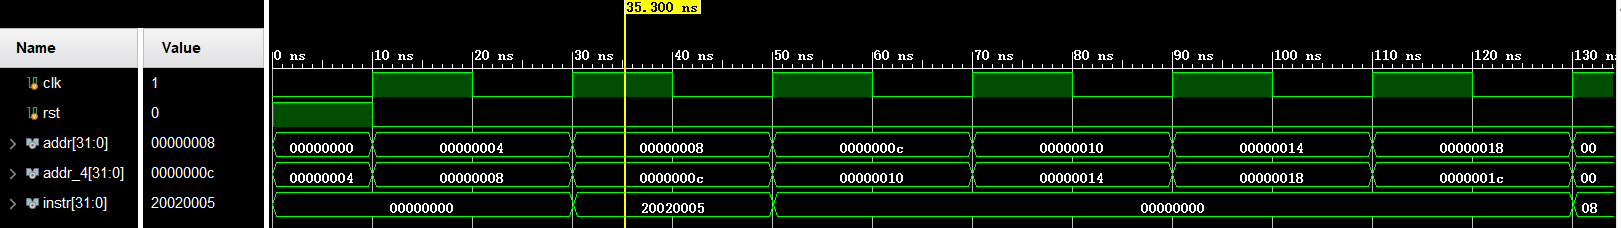
\includegraphics[width=0.8\textwidth]{wronginst.png}
    \caption{取指间断}
\end{figure}

\textbf{解决方案:}因为一开始添加的指令数很少,增加指令数后发现指令每四个取一次,所以猜测
该存储器的地址是字地址,将PC右移两位后,就能够连续取出指令

\subsubsection{问题2}
\textbf{问题描述:}在解决问题2的基础上,加入控制器进行仿真,发现alucontrol信号无法得到

\begin{figure}[htbp]
    \centering
    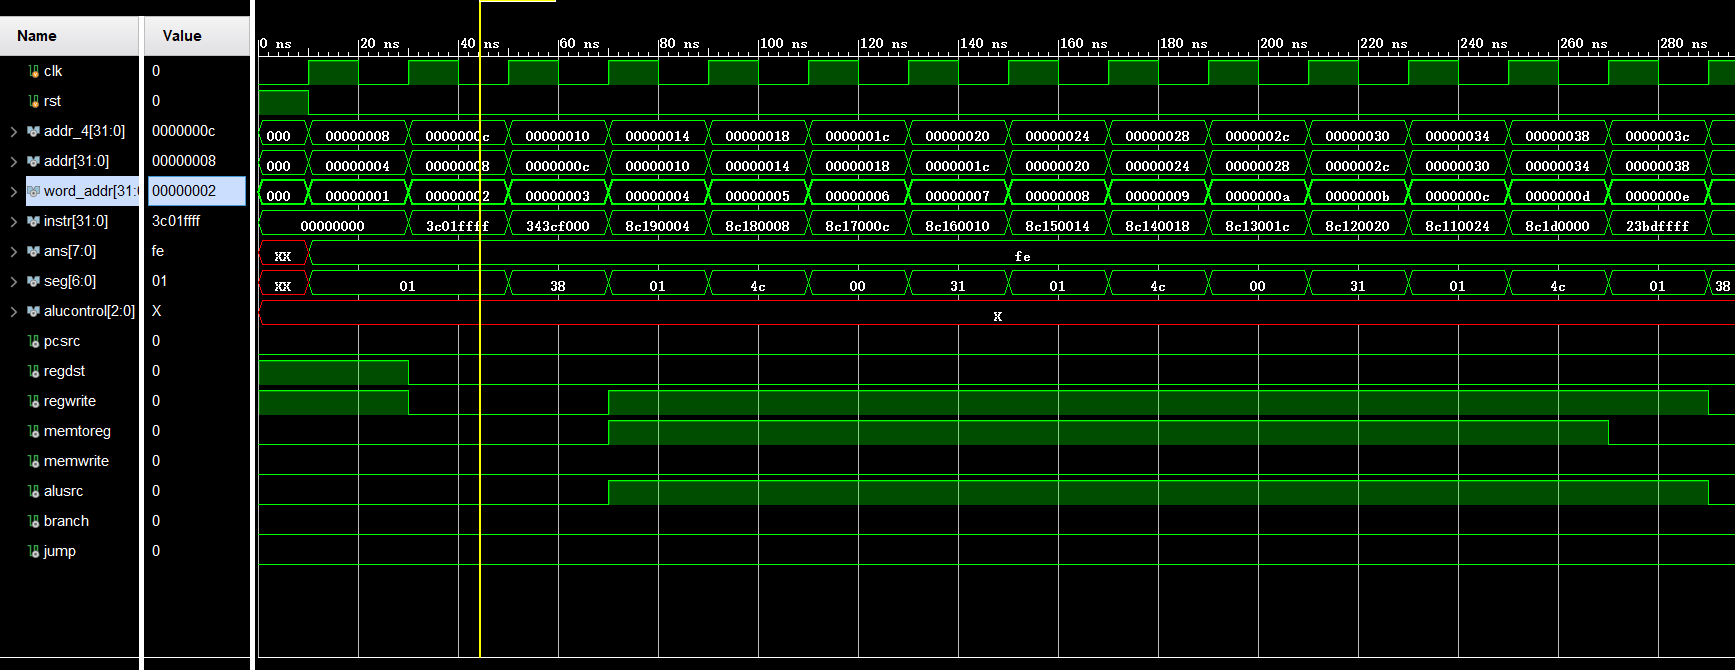
\includegraphics[width=0.8\textwidth]{wrongcont.png}
    \caption{Alucontrol错误}
\end{figure}

\textbf{解决方案:}在maindec和aludec中将aluop和alucontrol信号混淆,导致出现高阻态和未知态,交换位置后成功仿真